\documentclass[10pt]{article}
%%%%%%%%%%%%%%%%%%%%%%%%%%%%%%%%%%%%%%%%
\usepackage{amsmath}
\usepackage{verbatim}
\usepackage[usenames,dvipsnames]{color}
\usepackage{ulem}
\usepackage{setspace}
\usepackage{lscape}
\usepackage{longtable}
\usepackage[top=1.25in,bottom=1.5in,left=1in,right=1.5in,landscape]{geometry}
\usepackage{graphicx}
\usepackage{epstopdf}
\usepackage[usenames,dvipsnames]{pstricks}
\usepackage{epsfig}
\usepackage{pstricks-add}
\usepackage{pst-node}
\usepackage{fancyhdr}
\usepackage[absolute,showboxes]{textpos}

%TCIDATA{OutputFilter=LATEX.DLL}
%TCIDATA{Version=5.00.0.2552}
%TCIDATA{<META NAME="SaveForMode" CONTENT="1">}
%TCIDATA{Created=Thursday, August 28, 2003 13:38:44}
%TCIDATA{LastRevised=Thursday, August 14, 2008 15:20:27}
%TCIDATA{<META NAME="GraphicsSave" CONTENT="32">}
%TCIDATA{<META NAME="DocumentShell" CONTENT="Standard LaTeX\Blank - Standard LaTeX Article">}
%TCIDATA{Language=American English}
%TCIDATA{CSTFile=LaTeX article (bright).cst}

\setcounter{MaxMatrixCols}{10}

\newenvironment{proof}[1][Proof]{\noindent\textbf{#1.} }{\ \rule{0.5em}{0.5em}}
\setlength{\columnsep}{.2in}

\renewcommand{\labelitemii}{$\cdot$}

\pagestyle{fancy} \fancyhead{} \fancyfoot{} \rfoot{} \lfoot{}

\newcommand{\slide}[2]{
\begin{textblock}{11}(0,0)
\textcolor{Black}{\textbf{\huge \rule{0pt}{1in} \raisebox{.2in}{#1}}}
\end{textblock}
\begin{Large} \noindent
#2
\end{Large}
\vfill \pagebreak}

\setlength{\TPHorizModule}{1in}
\setlength{\TPVertModule}{1in}
\textblockcolour{Yellow}
\renewcommand{\headrulewidth}{0pt}



\begin{document}
\onehalfspacing 

\lfoot{Extensions of the Solow Model} \rfoot{Economic Growth}

\slide{Human Capital}{Modify the Solow model to include \textit{human capital}. This allows the skills of workers to increase, separately from technological progress.
\begin{equation}
Y = K^{\alpha}(AH)^{1-\alpha}
\end{equation}
where 
\begin{equation}
H = e^{\psi u}L.
\end{equation}

\vspace{.25in}\noindent $L$ is the number of workers. $u$ is the amount of time spent acquiring human capital (think of it as years of schooling).

\vspace{.25in}\noindent In per worker terms,
\begin{equation}
h = e^{\psi u}.
\end{equation} 

}

\slide{Return to $u$}{What is $\psi$? The increase in $H$ from one more unit of time acquiring human capital. Take total derivative:
\begin{equation}
dH = \psi e^{\psi u}L du = (\psi H) du 
\end{equation}
This is the absolute change in $H$ given an increase in $u$. The proportional change in $H$ is
\begin{equation}
\frac{dH}{H} = \psi du.
\end{equation}

\vspace{.25in}\noindent If $\psi = 0.10$, then this says that if $du = 1$, then $H$ rises by 10\%. This formula for human capital is consistent with micro-level evidence on wages and earnings. $\psi$ is the return to one year of schooling. 
}

\slide{The Modified Solow Model}{Start by writing output in per worker terms
\begin{equation}
y = k^{\alpha}(Ah)^{1-\alpha}.
\end{equation}
Take logs and derivatives,
\begin{equation}
\frac{\dot{y}}{y} = \alpha \frac{\dot{k}}{k} + (1-\alpha)\frac{\dot{A}}{A} + (1-\alpha) \frac{\dot{h}}{h}.
\end{equation}

\vspace{.25in}\noindent We assume that
\begin{eqnarray}
\frac{\dot{h}}{h} &=& 0 \\
\frac{\dot{A}}{A} &=& g
\end{eqnarray}
or human capital ($h$) does not have trend growth, but there is trend growth in technology ($A$).

\vspace{.25in}\noindent A balanced growth path, as before, is where $\dot{y}/y$ is constant. That required that $\dot{y}/y = \dot{k}/k$. So again we have that
\begin{equation}
\frac{\dot{y}}{y} = g
\end{equation}
along the balanced growth path. Human capital doesn't change this.
}

\slide{Steady state}{As before, along the balanced growth path $\dot{k}/k = g$. So in steady state 
\begin{equation}
g = s \frac{y}{k} - (\delta +n).
\end{equation}
Plug in for $y$ to get
\begin{equation}
g = s \frac{(Ah)^{1-\alpha}}{k^{1-\alpha}} - (\delta+n).
\end{equation}
Solve for
\begin{equation}
\frac{k}{Ah} = \left(\frac{s}{\delta +n +g} \right)^{1/(1-\alpha)}.
\end{equation}
}

\slide{Output per Worker Level}{Given 
\begin{equation}
\frac{k}{Ah} = \left(\frac{s}{\delta +n +g} \right)^{1/(1-\alpha)}.
\end{equation}
we know that
\begin{eqnarray}
y &=& Ah \left(\frac{k}{Ah}\right)^{\alpha} \\
y &=& Ah \left(\frac{s}{\delta +n +g} \right)^{\alpha/(1-\alpha)} \\
y(t) &=& A(t) e^{\psi u} \left(\frac{s}{\delta +n +g} \right)^{\alpha/(1-\alpha)}.
\end{eqnarray}

\vspace{.25in}\noindent We see here that human capital, as determined by $u$, influences the level of output per worker, even though it does not change the growth rate of output per worker. 

}

\slide{Relative Output per Worker}{Consider the model in relative terms. Relative to a rich-country standard like the U.S.
\begin{equation}
\hat{y}_i = \frac{y_i}{y_{US}}
\end{equation}
so that $\hat{y}_i$ is the output per worker of country $i$ relative to that in the U.S.

\vspace{.25in}\noindent If output per worker is described as in our modified model, then
\begin{equation}
\hat{y}_i = \frac{A_i e^{\psi u_i} \left(\frac{s_i}{\delta +n_i +g} \right)^{\alpha/(1-\alpha)}}{A_{US} e^{\psi u_{US}} \left(\frac{s_{US}}{\delta +n_{US} +g} \right)^{\alpha/(1-\alpha)}}.
\end{equation}
which can reduce to
\begin{equation}
\hat{y}_i = \frac{A_i}{A_{US}}e^{\psi(u_i - u_{US})}\left(\frac{s_i}{s_{US}} \right)^{\alpha/(1-\alpha)}\left(\frac{\delta+n_{US}+g}{\delta+n_i +g} \right)^{\alpha/(1-\alpha)}
\end{equation}

\vspace{.25in}\noindent Note, we've made the assumption that $g$ is identical for all countries.
}

\slide{Explaining Cross-Country Variation}{Solow originally assumed that $A$ was identical across countries, as they could share technology. How good does of a job does the model do if $A_i = A_{US}$?
\begin{equation}
\hat{y}_i = e^{\psi(u_i - u_{US})}\left(\frac{s_i}{s_{US}} \right)^{\alpha/(1-\alpha)}\left(\frac{\delta+n_{US}+g}{\delta+n_i +g} \right)^{\alpha/(1-\alpha)}
\end{equation}
Are the differences in $u$, $s$, and $n$ sufficient to explain cross-country output per worker differences?

\vspace{.25in}\noindent Plug in values of $\alpha = 1/3$, $\psi = 0.10$, $\delta +g = 0.075$. Use years of education as $u_i$. Use average savings rate as $s_i$. Use average population growth as $n_i$. 

\vspace{.25in}\noindent Example: $s_{India} = 0.241$, $u_{India} = 4.23$, $n_{India} = 0.017$. $s_{US} = 0.202$, $u_{US} = 13.24$, $n_{US} = 0.011$. So
\begin{equation}
\hat{y}_{India} = e^{0.10(4.23 - 13.24)}(0.241/0.202)^{1/2}(0.086/0.092)^{1/2} = 0.429
\end{equation}
Based on education, savings, and population growth, India should be 43\% as rich as U.S. India is actually about 9\% as rich as U.S. 
}

\slide{All Countries}{
\begin{center}
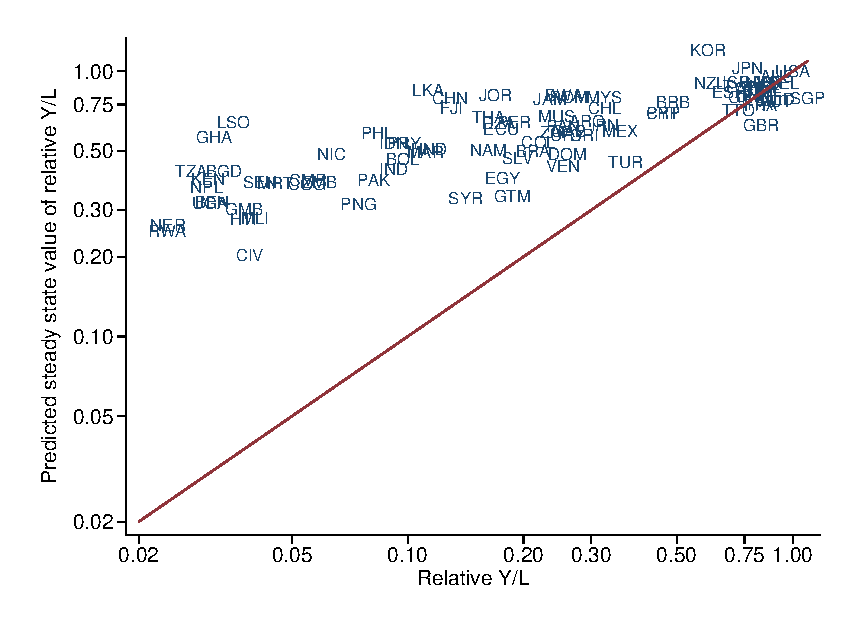
\includegraphics[scale=1.2]{figure_3_1.eps}
\end{center}
}

\slide{The Solow Residual}{Savings, education, and population growth do not explain all of the variation in output per worker. Those three factors suggest most poor countries should be much better off than they actually are. So what's missing?

\vspace{.25in}\noindent Technology/productivity differences. $A_i \neq A_{US}$ for countries. We cannot measure $A_i$ directly, but we can infer if from data. Take 
\begin{equation}
y_i = k_i^{\alpha} (A_i h_i)^{1-\alpha}
\end{equation}
and re-arrange to
\begin{equation}
A_i = \left(\frac{y_i}{k_i^{\alpha}h_i^{1-\alpha}}\right)^{1/(1-\alpha)}.
\end{equation}
Given data on $y_i$, $k_i$, and $h_i$ we can back out the actual value of $A_i$.

\vspace{.25in}\noindent The value of $A_i$ from this is sometimes called ``The Solow Residual''. It measures everything that matters besides $k_i$, $h_i$ for output per worker.

\vspace{.25in}\noindent Last, for comparison, calculate
\begin{equation}
\hat{A}_i = \frac{A_i}{A_{US}}
\end{equation}

}

\slide{Values of $\hat{A_i}$ across countries}{
\begin{center}
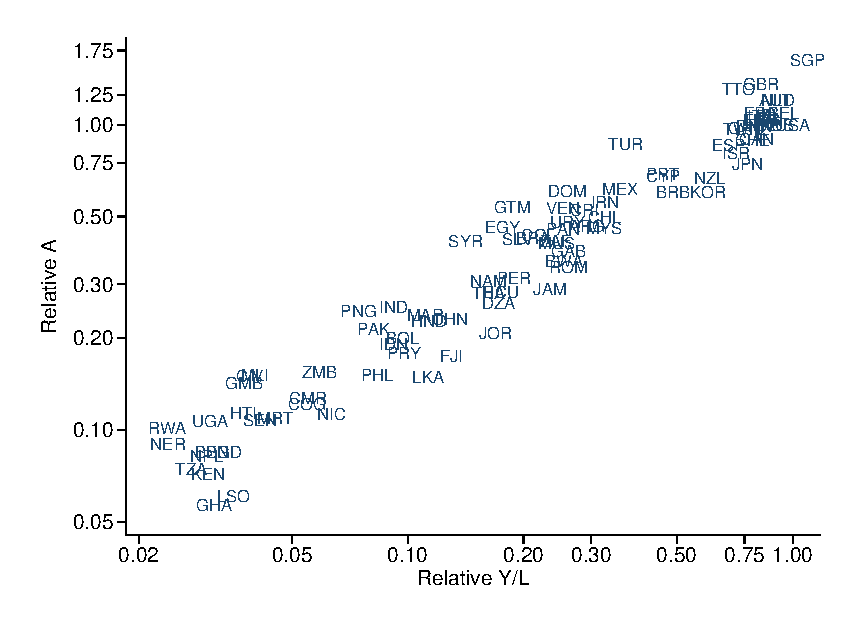
\includegraphics[scale=1.2]{figure_3_2.eps}
\end{center}
}

\slide{Technology Drives Differences}{The values of $\hat{A}_i$, by themselves, do a good job of describing differences in output per worker.

\vspace{.25in}\noindent Differences in $A_i$ explain about 1/2 to 2/3 of the differences in output per worker across countries. Why we will focus on explanations of the growth in $A_i$ and/or the level of $A_i$ rather than explanations of why $s_i$ or $n_i$ varies.

}

\slide{Growth Rate Differences}{Some countries grow more quickly than others. Why?

\vspace{.25in}\noindent One explanation: \textit{convergence}. Poor countries grow more quickly than rich countries. 

\vspace{.25in}\noindent Look at equation for growth rate of $\dot{k}/k$. 
\begin{eqnarray}
\frac{\dot{k}}{k} &=& s\frac{y}{k} - (\delta + n) \\
 &=& s\left(\frac{Ah}{k} \right)^{1-\alpha} - (\delta + n)
\end{eqnarray}
if
\begin{equation}
\frac{k}{Ah} < \left(\frac{s}{\delta +n +g} \right)^{1/(1-\alpha)}
\end{equation}
then $\dot{k}/k > g$. So if $k/Ah$ is low relative to steady state, country grows quickly.
}

\slide{Long-run Convergence}{Countries with similar $A$ and $h$:
\begin{center}
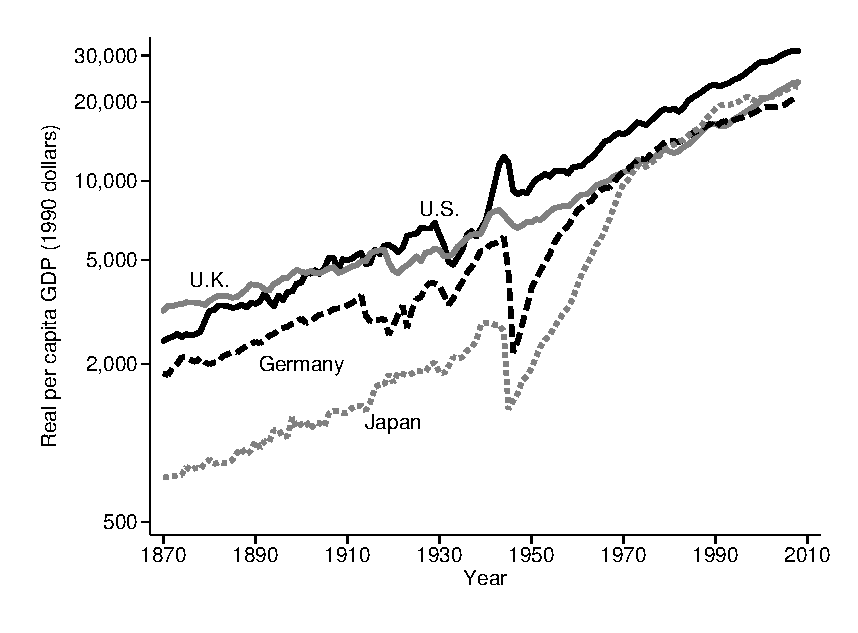
\includegraphics[scale=1.2]{figure_3_3.eps}
\end{center}
}

\slide{Long-run Convergence}{Countries with similar $A$ and $h$:
\begin{center}
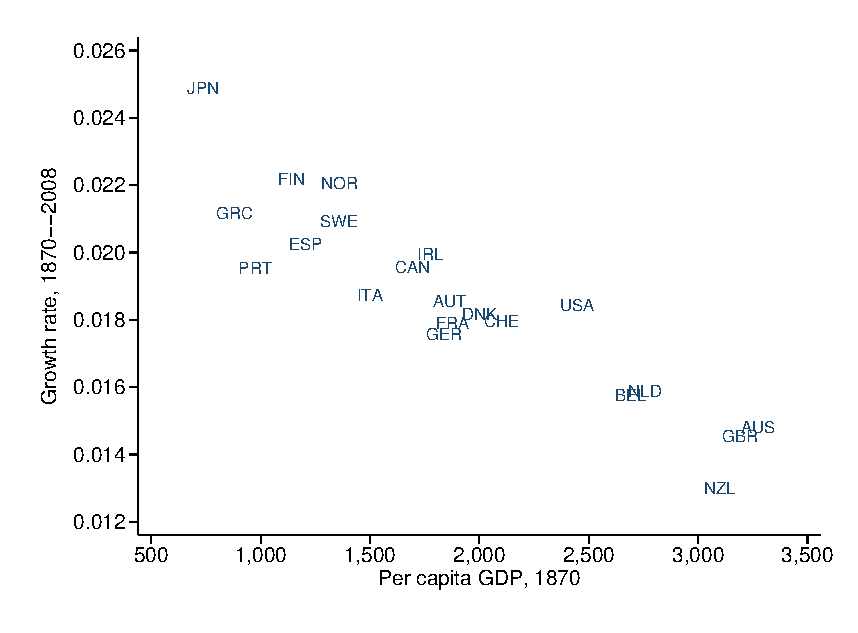
\includegraphics[scale=1.2]{figure_3_4.eps}
\end{center}
}

\slide{Convergence in the OECD}{Countries with similar $A$ and $h$:
\begin{center}
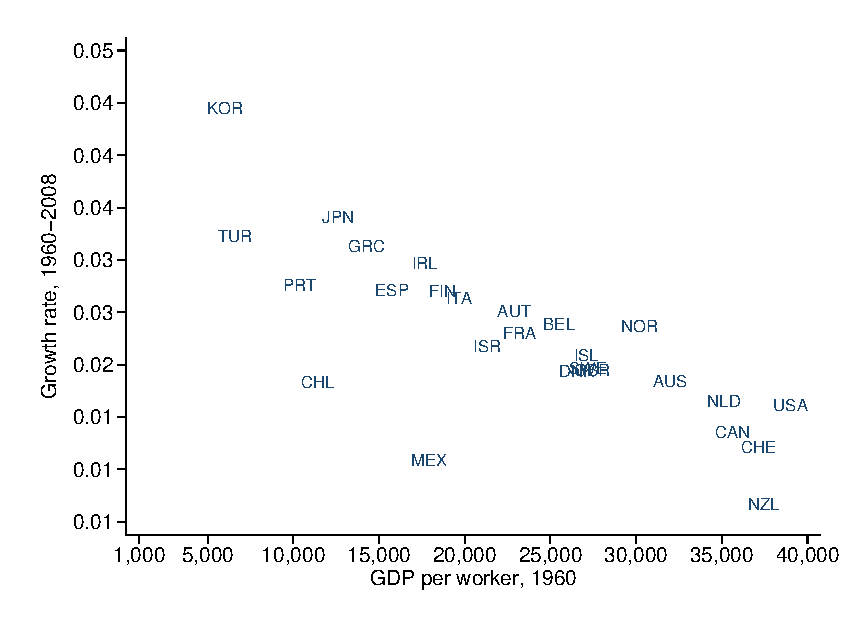
\includegraphics[scale=1.2]{figure_3_5.eps}
\end{center}
}

\slide{Lack of Convergence}{Countries with dis-similar $A$ and $h$:
\begin{center}
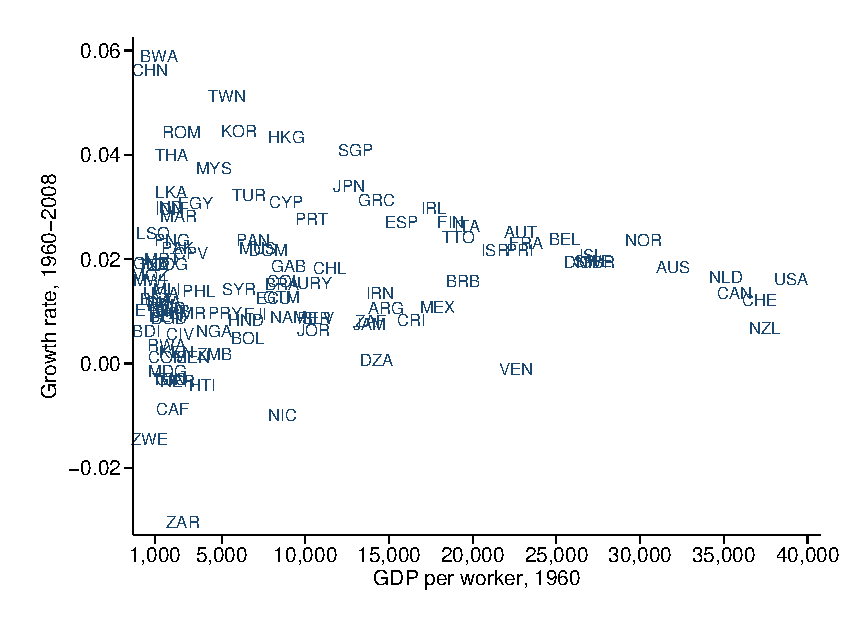
\includegraphics[scale=1.2]{figure_3_6.eps}
\end{center}
}

\slide{Conditional Convergence}{Not all countries seem to fit. They grow very slowly even though they are poor.

\vspace{.25in}\noindent Conditional convergence: countries grow faster, the farther they are \textit{from their own steady state}. Poor countries have low steady states, so they are already close to their steady state, and grow slowly.

\vspace{.25in}\noindent Can we see this in the data? Compute the steady state for each country as
\begin{equation}
y^{\ast}_i = A_{i} h_i \left(\frac{s_i}{\delta + g + n_i} \right)^{\alpha/(1-\alpha)}
\end{equation}
using data on $h_i$, $s_i$, and $n_i$ like before. Use the value of $A_i$ from 1970. 

\vspace{.25in}\noindent Then compute how far each country is from steady state
\begin{equation}
\frac{y_i}{y^{\ast}_i}
\end{equation}
and graph growth from 1960--2008 versus this relative value.

}

\slide{Lack of Convergence}{
\begin{center}
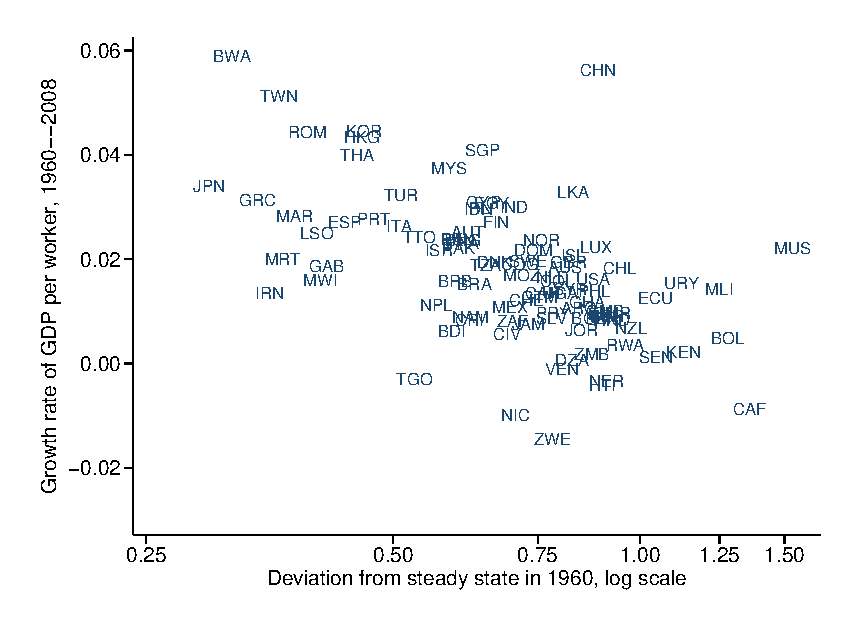
\includegraphics[scale=1.2]{figure_3_8.eps}
\end{center}
}

\slide{Equality?}{If there were absolute convergence (like in the OECD), then countries are getting more equal. If there is conditional convergence (like in the whole sample), then countries may be getting more unequal.

\vspace{.25in}\noindent In absolute numbers of people, world looks like it is getting more equal. Sala-i-Martin (2006): In 1970, 534 million people (15\% of world population) lived on less than \$1 per day. In 2000 only 321 million people (6\% of world population) lived on less than \$1. 

}

\slide{Lack of Convergence}{
\begin{center}
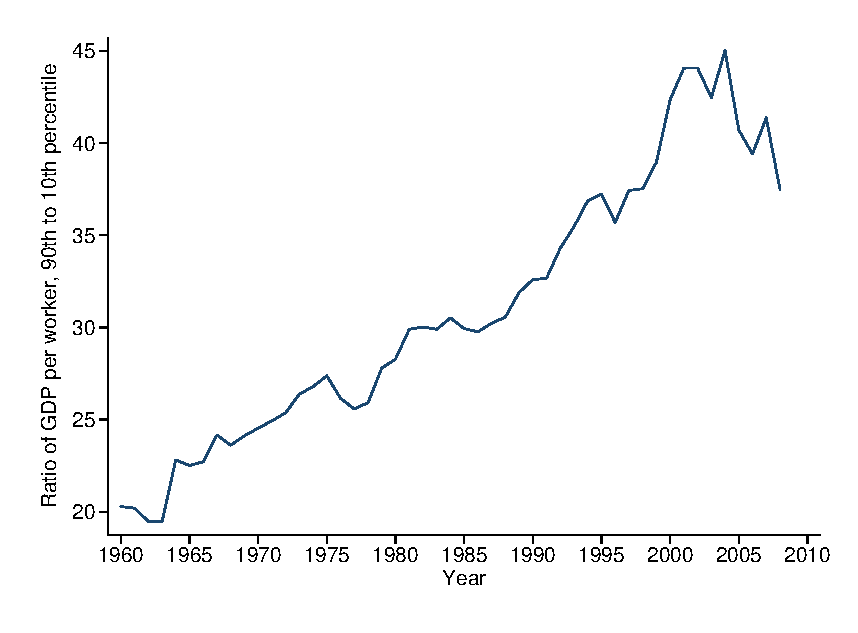
\includegraphics[scale=1.2]{figure_3_9.eps}
\end{center}
}

\slide{Lack of Convergence}{
\begin{center}
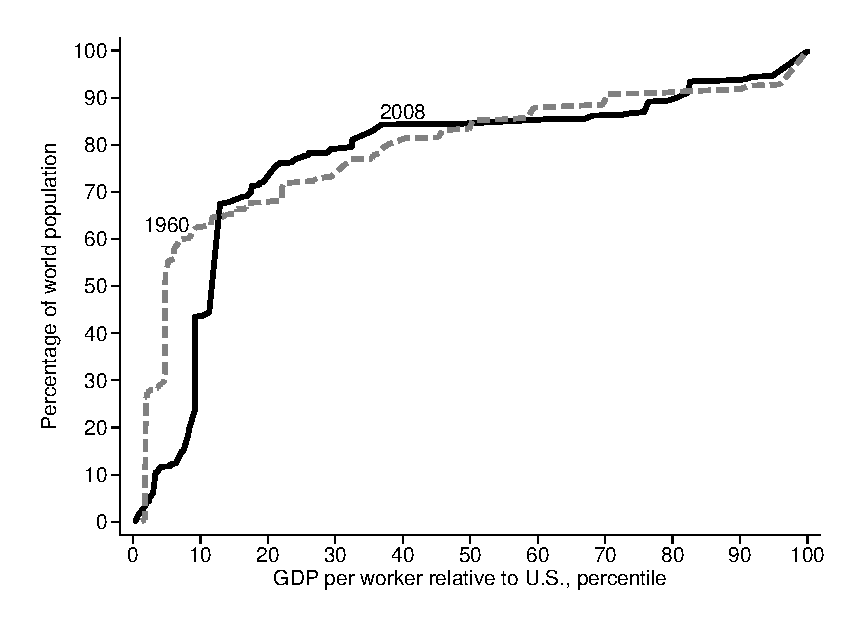
\includegraphics[scale=1.2]{figure_3_10.eps}
\end{center}
}


\end{document}